%
% Angol nyelvű szakdolgozat minta az Eszterházy Károly Egyetem hallgatóinak.
%

\documentclass[
% without options: one-sided printing, online version
% twoside,       % two-sided printing
]{thesis-ekf}
\setcounter{secnumdepth}{5}
\usepackage[T1]{fontenc}
\usepackage[english]{babel}
\usepackage{natbib}
\usepackage{lipsum}
\usepackage{pgfplots}
\usetikzlibrary{intersections}
\usepackage{csquotes}
\renewcommand{\mkbegdispquote}[2]{\itshape}
\usepackage{listings}
\usepackage{color}
\usepackage{subcaption}
\usepackage[colorinlistoftodos]{todonotes}
\usepackage{csquotes}

\definecolor{dkgreen}{rgb}{0,0.6,0}
\definecolor{gray}{rgb}{0.5,0.5,0.5}
\definecolor{mauve}{rgb}{0.58,0,0.82}

\lstset{frame=tb,
	language=Python,
	aboveskip=3mm,
	belowskip=3mm,
	showstringspaces=false,
	columns=flexible,
	basicstyle={\small\ttfamily},
	numbers=none,
	numberstyle=\tiny\color{gray},
	keywordstyle=\color{blue},
	commentstyle=\color{dkgreen},
	stringstyle=\color{mauve},
	breaklines=true,
	breakatwhitespace=true,
	tabsize=3
}
\usepackage{graphicx}
\graphicspath{{fig/}}





\begin{document}
	
	
\institute{Eszterhazy Karoly University}
\title{Machine Learning Model for Agricultural Data Applications}
\author{Adeyemo Adedeji Charles\\Computer Science BSc}
	
\supervisor{Bence Bogdandy\\Associate Professor
		\\bogdandy.bence@uni-eszterhazy.hu}
\city{Eger}
\date{2020/21}
\maketitle



\begin{abstract}
	Prediction of economical growth is a complex task which is essential for planning sustainable economy.	
	Economy has a wide range of indicators that are monitored and recorded by governments and international organizations, such as, the United Nations Food and Agriculture Organization.	
	Agricultural data set of the Food and Agriculture Organization has records on production of crops and other agricultural products whose production strongly relates to the Gross Domestic Product of many countries.
	
	
	Assuming that total crop production and agricultural economy growth are highly related, the production of crops and total value of income from agriculture can be learnt by sequential machine learning models.
	Recurrent Neural Networks excel in learning time series and sequential data. 
	This study presents experimental results on training various recurrent neural networks for predicting the Gross Production Value of a particular agricultural product - wheat - given certain data point parameters. 
	
	This predictive model also plays a role in the Hungarian economic policy as in the future it will serve a basis for the calculation of the expected income for a specific crop.
\end{abstract}

\chapter*{Dedication}

To my mentor and supervisor, Bogdandy Bence without whom this dream would have remained a dream. 

\tableofcontents

\chapter*{Introduction}

\todo{This is has to be concise. What is the purpose of my Thesis? What is the aim and the Objectives
for researching this particular area}

Gross Domestic Product (GDP) is one of the most popular economical term and parameter for the indication of the well-being of a country. It is used by governments and international organization for critical decision making based on the size and performance of an economy. So, it is very important to compute and measure it accurately. Having a precise measurement of GDP according to the defined way is essentially impossible because it's a quantitative value which doesn't take all social indicators into account.We are thus able to give an estimated, acceptable value of the GDP.

This work is based on how the GDP is affected. There are a number of factors which affects the GDP positively or negatively. These factors could be domestic or global. The internal factors include political conditions, the state of peace, government public policies, business policies etc. Global factor could be international relations with other nations, relations with the neighboring nations, distances from international markets and access to global markets. 


Exploring the history of economic and financial studies, it can be found that over 600 parameters can be identified \cite{richardson2020nowcasting} as predictors of GDP. After the innovation of this notion, its effectors have been analyzed in three distinct ways: qualitative analysis, statistical analysis and relational analysis. Qualitative analysis has often been the most popular in journalistic circles. While statistical analysis has been quite prevalent in economists circles. The use of machine learning is quite recent. It has made possible the exploration of several unanswered latent problems in economies.\cite{richardson2020nowcasting, milavcic2017application, kumar2019novel}


The objective of this research is to use predictive deep learning methods to study the impact of an agriculture crop, in this case wheat, on the economy of Hungary. It focuses on:

\begin{itemize}
	\item Period: \textbf{1961 - 2016}
	\item Crop: \textbf{Wheat}
	\item Data points: \textbf{Area, Quantity, Yield}
\end{itemize}

\textbf{Bence - input}Or it can be rewritten as: This research studies the effect of wheat production in Hungary between 1961 - 2016 and its direct effect on the Gross Domestic Product.

The rest of the document describes the role of neural networks in agricultural research. The methods of this proposed research are described in chapter II. After the comprehensive implementation in chapter III of the methods employed, the results of the works are discussed in chapters IV and V respectively.





\chapter{Related Works}
\todo{Also known as Literature. Concise. Here, I have to create a diagram that shows my thought process.}
\section{Data Science}
\todo{Create a Diagram and have my Question in the middle. From reading my first Journal paper, I'll add key branches to the diagram.}

\todo{In the diagram - Reader can identify - This is my Diagram - This is my Question and I have the relevant things properly cited and referenced. How to add citation to a diagram. }

\todo{So I'll talk about these themes from the Figure and how they are connected to my work. logically.Hence the Chapters bence said. This should be in the diagram.  }
Data Science encompasses making awesome visualizations and models using data. As a field of Computer Science, it has created as much positive impact in our society. Impact could be in the form of insights, in the form of data products or in the form of product recommendations for a company. In order to achieve these things, we need tools like writing code, machine learning models or data visualizations.


According to this article by Usama Fayyad \cite{fayyad1996data} data mining is referred to  as the overall process of discovering useful information from data. William S. Cleveland, \cite{cleveland2001data}   who at that time was a Distinguished Member of Technical Staff in the Statistics Research Department at Bell Labs, Murray Hill, defined data science as it is used today. He did that by combining computer science with data mining. He made statistics a lot more technical because he believed it would expand the possibilities of data mining and produce a powerful force for innovation. Now, we can take advantage of computational power for statistics.



\subsection{Technical Advancement}
Around this time, \textbf{web 2.0} emerged. Websites aren't simply digital pamphlets anymore, but a medium for shared experience among millions of users. These are websites like:
\begin{itemize}
	\item \textbf{MySpace:} 2003
	\item \textbf{Facebook:} 2004
	\item \textbf{YouTube:} 2005	
\end{itemize}

As users, we can now interact with these websites - post, comment, share - leaving our digital footprints on the Internet. That's a lot of data and soon enough, it became too much to handle using traditional technologies. This opened a world of possibilities in finding insights using data. So the rise in data sparked the rise of data science to support the needs of businesses to draw insights from their massive unstructured data sets. This abundance of data now makes it possible to train machines with a data-driven rather than a knowledge-driven approach. Deep learning is no longer an abstract academic concept in this thesis paper. It is a tangible useful class of machine learning model for agricultural data applications.

\section{Machine Learning Workflow}
From predicting economic growth to detecting cancers, Machine Learning has granted computer systems entirely new abilities. The first step to solving a Machine Learning task is to define the problem and assemble a data-set. The data-set has to be one with integrity. Choosing a measure of success and deciding on a validation protocol are the next logical steps. The most important step in building a Machine Learning model is the preparation of the data. It won't occur in a real-life situation that raw data is ready to be fed into a machine model. 

Once the data is ready, the model can be built. At first, we build one that over-fits. Afterwards this model is regularized and its hyper-parameters tuned. 

\begin{figure}[h!]
	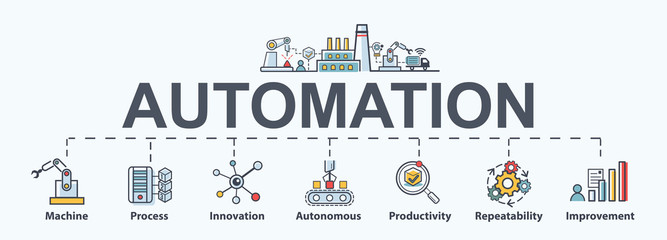
\includegraphics[width=\textwidth,height=\textheight,keepaspectratio]{workflow.png}
	\caption{Machine Learning Workflow.}
	\label{fig:workflow}
\end{figure}

Figure \ref{fig:workflow} shows the workflow of a typical Machine Learning model.



\chapter{Methods}
\section{Data Science}

\todo{It's critical that this section JUSTIFIES THE TOOLS I'm using. Think of a plumber.}

\todo{I'll have to JUSTIFY my approach}

\todo{I'll have to justify why I am selecting certain tools to answer my Research questions. That is the questions in the Diagram in Related Works}

\todo{In addition, extract questions that go into a table. Justify why you have selected the sections and reference the Literature review. Maybe not relevant to my work.}

Data Science is a subset of Computer Science and Mathematics. This subset introduces a new paradigm which creates algorithms for computers and robots. Data Science also involves the use of machine learning algorithms for prediction.


In the field of Data Science, mathematics is very important. This is because principles within mathematics help in the detection of patterns and algorithm construction. In the application of such algorithms in data science, the comprehension of different conceptions of statistics and probability theory is crucial. Notions include Regression, Maximum Likelihood Estimation, distribution's comprehension (Binomial, Bernoulli, Gaussian (Normal)), and Bayes's Theorem.

The foundation of every current field of science is mathematics. Almost all data science methods have a strong mathematical underpinning, like machine learning.
It comes as no surprise that to work as a top data scientist, you would completely need all the other beads of expertise-programming ability, some volume of business intelligence, and your unique analytical and curious mentality-about the data. But learning the machinery under the hood is still worth it, instead of just being the guy behind the wheel with no understanding of the car. A good awareness of the mathematical machinery behind the trendy algorithms would also give you an advantage over your colleagues.

\section{Machine Learning}

Machine Learning is a novel part of Data Science and it encompasses the ability of machines to learn from examples. These models are categorized as either \textbf{\textit{Supervised}} or \textbf{\textit{Unsupervised}} Machine Learning models. 

\subsection{Supervised Learning}
Supervised learning is essentially a formalization of the notion of learning from formerly supervised fields of learning. The learner (usually, a computer programme) is presented with two data sets, a training set and a test set during supervised learning. The idea is to set the learner's training set test to learn 'from a set of classified examples in the training set such that unlabeled examples can be defined with the greatest expected precision in the test set. That is, the learner's goal is to create a law, a programme, or a process that classifies new examples by evaluating examples that already have a class \cite{learned2014introduction}

Supervised learning is further categorized as  either \textbf{\textit{Regression}} or \textbf{\textit{Classification.}} The main difference between Regression and Classification is that the output variable in Regression is numerical while that for Classification is categorical. In other words, Regression predicts a quantity while  Classification predicts a label.


\subsubsection{Machine Learning model - Regression}
In this 1998 article, \cite{zeger1988regression} Scot Zeger posits the analysis of a regression model with a time series. Linear Regression is a basic offshoot of Regression. The predicted output of a Linear Regression model is continuous with a constant slope. The 2 main types of Linear Regression are simple and multivariate regression. 

Simple linear regression can be explained with the slope-intercept form, where \textit{m} and \textit{b} are the variables the algorithm learns to produce the most accurate predictions. \textit{x} in this case represents the input data while \textit{y} the prediction.

\begin{equation}
	y = m x + b
\end{equation}

Multivariate regression is a method with more than one output variable that calculates a single regression model. If a multivariate regression model has more than one predictor variable, the system is a multivariate multiple regression.

A natural extension of multiple linear regression is multivariate linear regression in that both methods aim to explain hypothetical linear correlations between some variables of outputs and inputs. Multiple regression is focused on the analysis of the degree to which a set of "i" input variables X= (X1,Xi) influences the behaviour of a single output variable Y. The multivariate regression has "o" output variables Y= (Y1,Yo), each of which can be affected by precisely the same range of X= (X1,Xi) inputs.\cite{izenman2013multivariate}


\subsubsection{Machine Learning model - Classification}

In this 2006 paper by Kevin P. Murphy \cite{murphy2006naive} he defines a \textbf{classifier} as a function \textit{f} that maps input feature vectors to output classes. This classifier is derived from the \textbf{Bayes' Theorem}

A classification is a tool used to assign groups to a data set in order to assist in detailed forecasts and analysis. You are introduced to an existing data-set with classification algorithms and are aware of the groups of individual instances; with this information, a predictive model can then be created to solve the following problem: For any future instance in the data-set to which a particular instance belongs. Max Entropy, K-Nearest Neighbor, and Naive Bayes are among the types of classification algorithms.



\begin{equation}
	\label{eq:bayes}
	P(\theta | \textbf{D}) = P(\theta ) \frac{P(\textbf{D} |\theta)}{P(\textbf{D})},
\end{equation}



\subsection{Unsupervised Learning}
Unsupervised learning is a category of ML methods that work in the dataset of unlabeled data in order to explore frameworks or trends. New paradigms for unsupervised learning (as such-called self-supervised learning) have also been introduced to manipulate multiple labels that are readily accessible to learn general purpose characteristics in addition to or within visual data.\cite{dayan1999unsupervised}
Unsupervised learning explores how models should learn in a way that illustrates the mathematical form of the overall input sequence set to describe individual input sequence. In comparison to supervised learning or reinforcement learning, each feedback is not correlated with specific goal outcomes or environmental assessments; instead, the unsupervised learning incorporates previous prejudices as to what elements of the input system can be reflected in the output.\cite{dayan1999unsupervised}



\section{Machine Learning Workflow}
One of the fundamental goals of Data Engineering is to develop data pipelines. A Data pipeline means taking data from point A (in an operational system) and then moving it to point B (into something that can be analyzed by data scientists).
The data set used for this thesis paper was gotten from the Food and Agriculture Organization of the United Nations. This organization is tasked with creating a zero-hunger World. Starting from 1945, this organization has amassed a wealth of data-set archives from its member countries all over the world. My focus is on Hungary thus, making my contribution to creating a zero-hunger Hungary.

According to the official website,\cite{division_2000}
\begin{displayquote}
	"FAOSTAT provides free access to food and agriculture data for over 245 countries and territories and covers all FAO regional groupings from 1961 to the most recent year available."
\end{displayquote} 

To achieve my goals I focused on the \textbf{Value Of Agricultural Production} and in particular the \textbf{Gross Production Value.} This value was gotten by multiplying agricultural gross production by the output prices. In the data-sets used in this thesis paper, the gross production value is expressed in US dollars. 



Different data sets are available separately. For the purpose of this thesis, I narrowed down on wheat. I adopted a consistent time-frame. 1965 to 2002. The approach to this was: Given a set of features that are consistent with a particular agricultural product, the aim is to predict the Gross Production Value.

\section{Neural Networks}
A neural network is a collection of algorithms that, through a mechanism that mimics the way the human brain works, aim to identify fundamental connections in a data set \cite{jain1999recurrent}.  Neural networks, in this context, apply to neuron frameworks, either biological or artificial in nature. 

\subsection{Biological Neural Network}
Neural networks may respond to evolving inputs, so the network delivers the best possible outcome without the performance parameters having to be revamped. In the development of trading systems, the notion of neural networks, which has its origins in artificial intelligence, is rapidly gaining prominence.\citealp*{krose1993introduction}.


The biological neuron relations are modeled as weights. An excitation relation is reflected by a positive weight, whereas negative values mean inhibitory connections. Each input is updated and summarized by a weight. A linear combination is related to this practice. Finally, the amplitude of the output is regulated by an activation function. A reasonable performance range, for example, is usually between 0 and 1, or it may be −1 and 1.

\subsection{Artificial Neural Network}

To be developed.

\section{Deep Neural Network}

A recurrent Neural Network(RNN) is a type of Neural Network in which the previous phase output is fed to the current stage as an input. Both the inputs and outputs are independent of each other in conventional neural networks, but in situations such as where it is important to predict the next word of a sentence, the prior words are needed and so the past words need to be recalled. RNN thus came into being, which, with the aid of a Hidden Layer, fixed this problem. Hidden State, which recalls any details about a sequence, is the key and most significant aspect of RNN.\cite{jain1999recurrent}

By giving all layers the same weights and preferences, RNN transforms the independent activation into dependent activation, thereby reducing the difficulty of increasing parameters and memorizing each previous output by giving each output to the next hidden layer as an input.
Therefore, all three layers should be merged into a single recurring layer such that the weights and biases of all the hidden layers are the same.

The formula for calculating the current state:

\[Ht = f(ht-1, Xt)\]

\textit{where} \textbf{H} is the current state, \textbf{ht-1} is the previous state and \textbf{Xt} is the inpunt state.

\subsection{GRU}  % DOn't Touch
\subsection{LSTM}
What is LSTM: It's the \textbf{Long short Term Memory} This networks rely on a gated cell to track information throughout many time-steps. How do LSTM work?

\begin{itemize}
	\item Forget: The lSTM forget their irrelevant history.
	
	
	\item Store: They perform computation to store relevant parts of new information.
	
	
	\item Update: They use the above items 1 and 2 to update their internal state.
	
	
	\item Output: Finally, they generate an output.
\end{itemize}

In summary, LSTMs help with uninterrupted gradient flow.

Testing my commit

\section{Deep Learning}
\subsection{Machine Learning vs Deep Learning}



\chapter{Implementation}
\section{Data Science - Engineering}
\todo{Demonstrate the ability for analysis.}
\todo{Link to Related works - Not repeating. Might look at the sections and link them}

\todo{Section 1 is very interesting and further supports, or cast doubts or raises question marks about what is being said in the Related works.}
The process of collecting raw data from sources, transforming it so that it matches our system's requirements and loading it into a data-set is know as \textbf{ETL.} This \textit{acronym} represents \textit{Extract - Transform - Load.}

\begin{figure}[h!]
	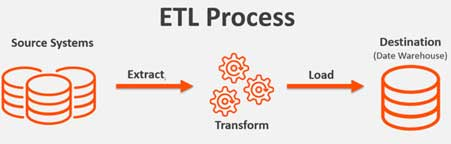
\includegraphics[width=\textwidth,height=\textheight,keepaspectratio]{fig/etl.jpg}
	\caption{Extract Transform Load.}
	\label{fig:ETL}
\end{figure}

Figure \ref{fig:ETL} shows the ETL process.


This raw data set contains lots of columns which are not necessary. The next step will be to clean the data by dropping these unnecessary columns. 


\subsection{Data Extraction.}

As mentioned in the previous chapter, the source of data for the purpose of this thesis was the Food and Agriculture Organization of the United Nations. To achieve my goals I focused on the \textbf{Value Of Agricultural Production} and in particular the \textbf{Gross Production Value.} This value was gotten by multiplying agricultural gross production by the output prices. In the data-sets used in this thesis paper, the gross production value is expressed in US dollars. 


Different data sets are available separately. For the purpose of this thesis, I narrowed down on wheat. I adopted a consistent time-frame (\textbf{1965 to 2002}). The approach to this was: \textit{Given a set of features that are consistent with a particular agricultural product, the aim is to predict the Gross Production Value.}

To make the downloaded data set globally available, I uploaded it to my GitHub repository.\cite{adeyemo_2020}

\begin{lstlisting}[language=Python]
	url_wheatArea = 'https://raw.githubusercontent.com/k-plasma/Machine-Learning-Models-for
	-Agricultural-Data-Applications/master/wheatArea.csv'	
	
	url_wheatGrossProduction = 'https://raw.githubusercontent.com/k-plasma/Machine-Learning-Models-for
	-Agricultural-Data-Applications/master/wheatGrossProductionValue.csv'	
	
	url_wheatProductionQuantity = 'https://raw.githubusercontent.com/k-plasma/Machine-Learning-Models-for
	-Agricultural-Data-Applications/master/wheatProductionQuantity.csv'	
	
	url_wheatYield = 'https://raw.githubusercontent.com/k-plasma/Machine-Learning-Models-for
	-Agricultural-Data-Applications/master/wheatYield.csv'
\end{lstlisting}

\begin{figure}[h!]
	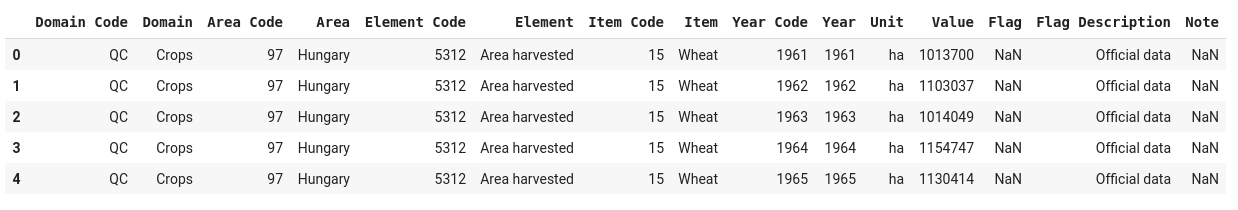
\includegraphics[width=\textwidth,height=\textheight,keepaspectratio]{fig/Area_Head.png}
	\caption{Raw Data Area.}
	\label{fig:Areaa_Head1}
\end{figure}

Figure \ref{fig:Areaa_Head1} shows the top 5 rows of the Data Set.


Each set of data set contained lots of columns which are repetitive and irrelevant to the task at hand. These columns include: \textit{"Domain Code","Domain",
	"Area Code","Area","Element Code","Element","Item Code","Item",
	"Year Code","Unit","Flag","Flag Description","Note"}

\subsection{Data Cleaning} 
The repetitive columns constitute noise which isn't required. I drop these to narrow down on the vital data necessary for my task. Two columns are left: \textit{"Year", "Value".} Since the word \textit{"Value"} appears in the different data-sets, it's renamed here as \textit{"Area(Hectares)"} to clearly indicate that this value refers to the measurement of the area.


\begin{lstlisting}[language=Python]
	df_wheatArea.drop(columns=["Domain Code","Domain",
	"Area Code","Area","Element Code","Element","Item Code","Item",
	"Year Code","Unit","Flag","Flag Description","Note"], axis=1, inplace=True)
	
	df_wheatArea.columns = ['Year', 'Area(Hectares)'] 
	
	df_wheatArea.head()
\end{lstlisting}

A similar transformation is performed on the other data-sets. The resulting individual data-sets are: 
\begin{figure}
	\centering
	\begin{subfigure}{.25\textwidth}
		\centering
		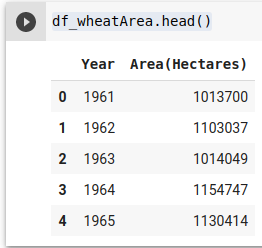
\includegraphics[width=.4\linewidth]{fig/areaHectares.png}
		\caption{Area}
		\label{fig:sub1}
	\end{subfigure}%
	\begin{subfigure}{.24\textwidth}
		\centering
		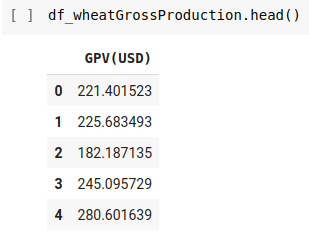
\includegraphics[width=.4\linewidth]{fig/gpv.png}
		\caption{G.P.V}
		\label{fig:sub2}
	\end{subfigure}
	\begin{subfigure}{.25\textwidth}
		\centering
		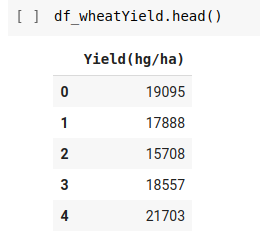
\includegraphics[width=.4\linewidth]{fig/yield.png}
		\caption{Yield}
		\label{fig:sub3}
	\end{subfigure}
	\begin{subfigure}{.24\textwidth}
		\centering
		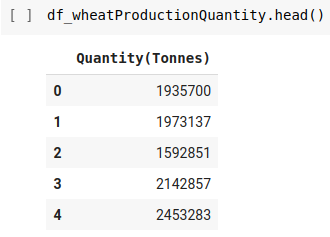
\includegraphics[width=.4\linewidth]{fig/quantityTonnes.png}
		\caption{Quantity}
		\label{fig:sub4}
	\end{subfigure}

	\caption{Individual Transformed Data-Sets}
	\label{fig:heads}
\end{figure}



\section{Implementing Machine Learning Work Flow}





\subsection{Assembling the Data Set}
\section{How I implemented the Neural Networks}
\section{Recurring Neural Network}
\section{Deep Learning}

\chapter{Results}
\section{Neural Networks}
In this section, I will describe the Progression from Normal Neural network to Recurring Neural Networks - RNN. In the end, I'll show that the GRU works well and I have solved what I set out to do. 
it should be here
\subsection{Subsection title}
Neural Networks and more advanced technologies. Right now we use Pandas for everything and it's enough, except when it's not. The more advanced we go into tech, the more basic the Machine Learning tools.

Some Machine Learning models are very dependent on used materials. SCI-KIT uses the most basic of Neural networks. What you'll notice from GPV-Take 1 is that you can't create modern systems with SCI-KIT because it is the highest level of abstraction.

Here, I'll need to show the results of the Google Colab Notebook - Gross Production Value 1 and the abysmal results I got using SCI-KIT

We use SCI-KIT for scaling. It implements it very well. Train - Test - Split
\cite{ponce1989engineering}



\chapter{Discussion}
\section{Section title}

In this work, an estimated relationship between wheat crop of Hungary and its GDP (indicated with GVP) is established. The work is inspired by extensive literature reviews and some previous related studies. In some of the studies artificial neural networks (ANN) were extensively used. It has been shown that recurrent networks, specifically its variants LSTM and GRU can perform much better. This can be verified comparing the results of FFNNs and RNNs in Figure ~\ref{fig:feedforward} and Figure ~\ref{fig:trg}. 

Although the results from GRU are promising, but it poses the challenge of training the network appropriately. Specifically, how the speed and accuracy can be balanced and made optimum. With all of its pros and cons, it has been able to cater to the problems dynamically and actively. Also, these networks can be employed to solve huge sets of problems. 

From the results in Figure ~\ref{fig:trg}, it can be concluded that wheat quantity and wheat yield can significantly affect the GDP. This is particularly true since a large number of other agriproducts are directly dependent on wheat production. If the wheat yield is good enough, it can not only meet the requirements of food, but it can help flourish several related food industries. These two factors can significantly contribute to the country GDP. Also, they can help boom the exports sector of the economy. 
\subsection{Subsection title}




\chapter{Summary}

\section{Section title}
\subsection{Subsection title}

\todo{What are the general findings of the Research?}
\todo{What are the implications for the Government as per Economic planning}


\todo{Add a Recoomendation Chapter. This is my contribution to the industry.}

\todo{In Recomendation, maybe create another diagram like a Food pyramid.?? wtf}







\bibliographystyle{plain}
\bibliography{reference}
\end{document}
